%%%% Header %%%%%%%%%%%%%%%%%%%%%%%%%%%%%%%%%%%%%%%%%%%%%%%%%%%%%%%%%%%%%%%%%%%

\documentclass[12pt, parskip=half]{scrartcl}

\usepackage{jonas}

\bibliography{/home/jon/lucile/share/Dropbox/sci/refs/mendeley_bibtex/2016-09-imort_selection.bib}
\hyphenation{}

%%%% Meta data %%%%%%%%%%%%%%%%%%%%%%%%%%%%%%%%%%%%%%%%%%%%%%%%%%%%%%%%%%%%%%%%

\usepackage[
  pdfauthor   ={Jonas Schöley},
  pdftitle    ={Selection and Adaptation Components of Infant Mortality},
  pdfsubject  ={},
  pdfkeywords ={},
  pdfproducer =Latex,
  pdfcreator  =pdflatex
]{hyperref}

\title{Selection and Adaptation Components of Infant Mortality}
\author{
  Jonas Schöley\thanks{Max-Planck Odense Center on the Biodemography of Aging, University of Southern Denmark.}
  \and
  James Oeppen\footnotemark[1]
  \and
  Rune Lindahl-Jacobsen\footnotemark[1]
  \and
  James W.~Vaupel\thanks{Max Planck Institute for Demographic Research, Rostock, Germany.}~\footnotemark[1]
}

%%%% Titlepage %%%%%%%%%%%%%%%%%%%%%%%%%%%%%%%%%%%%%%%%%%%%%%%%%%%%%%%%%%%%%%%%

\begin{document}

\maketitle

\thispagestyle{empty}

\begin{abstract}
We test the selection hypothesis of infant mortality against the adaptation hypothesis by decomposing the mortality age pattern over the first year of life into an adaptation- and a selection component.  We show that the population level decline in mortality over the first hour of life is significantly influenced by mortality selection, i.e.~the frailest infants leaving the population shortly after birth. The subsequent mortality decline predominantly results from mortality changes observed in homogeneous sub-populations. This confirms the common view of the infant mortality age pattern being caused by adaptation on an individual level. The analysis is informed by detailed micro-data on births and infant deaths in the United States including more than 25 million births and 162,546 deaths. No parametric assumptions were necessary.
\end{abstract}

\clearpage

%%%% Text %%%%%%%%%%%%%%%%%%%%%%%%%%%%%%%%%%%%%%%%%%%%%%%%%%%%%%%%%%%%%%%%%%%%%

The age pattern of infant mortality is commonly described as resulting from an \emph{adaptation process}. As the infant ages, it grows and acquires robustness, continuously increasing its resilience against death. The parametric mortality models by Siler (1979) and by Heligman and Pollard (1980) are examples of this line of thinking.\footnote{
  \emph{\enquote{C measures the rate of mortality decline in childhood (the rate at which a child adapts to its environment)}} (\cite{Heligman1980}). \emph{\enquote{While the most common use of this decreasing hazard would be to account for the hazard due to immaturity, it can also be used [$\ldots$] for other hazards to which an animal adjusts successfully}} (\cite{Siler1979}).
}
An alternative explanation frames the declining force of mortality in early life as a \emph{selection process}. Infants who are born unfit for life will contribute heavily to the mortality rates observed right after birth. Due to this selection the mortality rate of the population will over time converge to the low-levels of the healthy survivors. These ideas can be formally expressed via the \enquote{frailty model}, a random effects proportional hazards model originally devised by \cite{Vaupel1979} in order to explain the old-age mortality deceleration. Various authors point to mortality selection as an explanation for the age pattern of infant mortality: \cite{Hougaard1984} points out that infant mortality can be modelled in a proportional hazards framework with a frailty factor $z$ coming from a distribution exhibiting extremely large variance and thereby capturing the inherent survival differences between infants born healthy and infants born with severe congenital disorders; \cite{Vaupel1985} show that two sub-populations with an age-constant hazard of differing magnitude will produce a declining hazard if grouped together; \cite{Levitis2011} explicitly names the \emph{heterogeneous frailty hypothesis} as a possible basis for the declining mortality before senescence. As of now however, the selection hypothesis remains untested.

\begin{figure}[!htb]
  \centering
  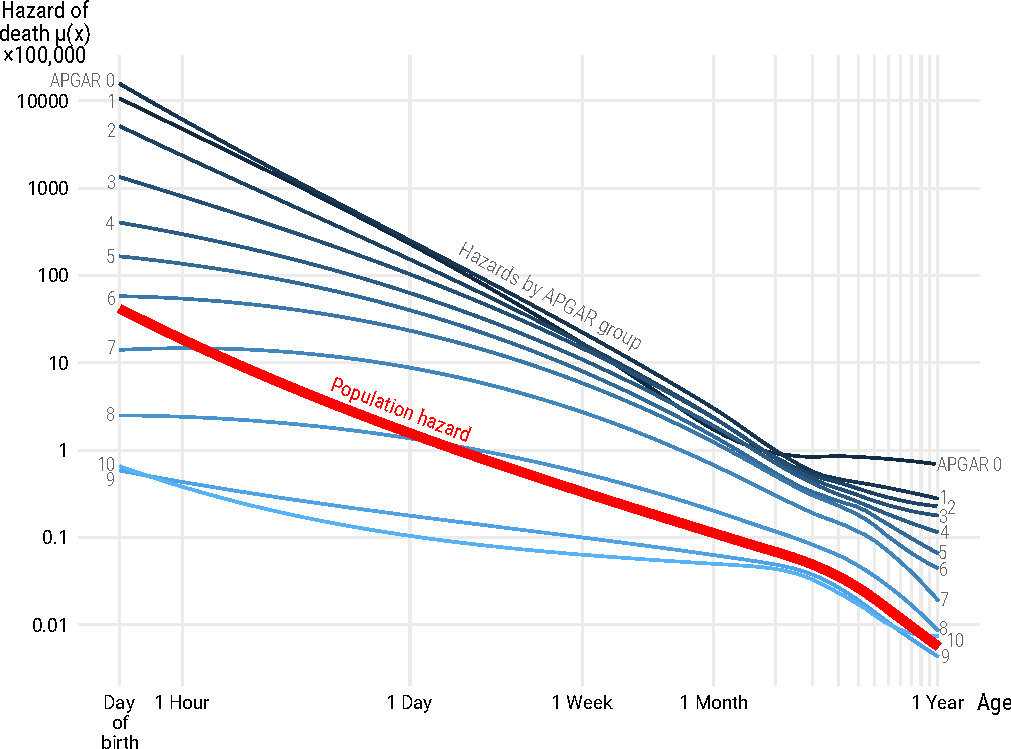
\includegraphics[width = \textwidth]{./fig/plot_ilt_dob0510_apgar5.pdf}
  \caption{Hazard of death over the first year of life for infants born in the US 2005--10 by 5 minute APGAR score and on aggregate. All APGAR groups experience some degree of mortality decline though the shape and speed of that decline varies. The effect of mortality selection can clearly be seen by the population hazard approaching the hazard of the high-APGAR groups (e.g. those with a survival advantage). The hourly/daily mortality rates have been \textsc{loess}-smoothed prior to plotting. Data: Calculated on the basis of the birth cohort linked birth-infant death data files by the National Center for Health Statistics.}
  \label{fig:apgar}
\end{figure}

We use an equation from evolutionary biology, coupled with vast and detailed individual level data on infant mortality, to precisely answer what proportion of an observed age-decline of mortality is explained by adaptation, and what proportion by mortality selection.

The \enquote{Price-equation} (\cite{Price1970}) allows to decompose how much of an observed change in a phenotypic trait between two generations is due to a \enquote{real} change in the trait between parents and offspring and how much is due to selection by trade-specific reproduction rates. \cite{Vaupel2002} and \cite{Vaupel2010a} independently derived this equation in the context of frailty models and mortality selection, decomposing the change of an average hazard of death into the average change of individual hazards minus the variance of the individual hazards, or, in the context of infant mortality, the adaptation and the selection component:

\begin{equation}
  \dot{\bar{\mu}}(x) = \bar{\dot{\mu}}(x) - \sigma^2_\mu(x)
  \label{eq:dec}
\end{equation}

Of course an individuals hazard of death can't be measured by mortality rates as the latter are only defined on a group of people. However, the individual hazards can be approximated by mortality rates calculated for a homogeneous group, i.e.~a group where all the members feature the same mortality relevant co-variates such as sex, birth-weight, age of mother, congenital malformations, etc. In the first analysis presented here we use the \emph{APGAR} score, one of the best predictors for the risk of infant death, as the variable constituting homogeneous groups. The APGAR score measures the overall vitality of a newborn on a scale from 0 (no vital signs) to 10 (strongest vital signs) and can be regarded as a very good proxy for the (inverse-) frailty of a child. Using publicly available microdata on live births and infant deaths in the United States provided by the National Center for Health Statistics we calculate life-tables over day of age for each of the APGAR scores.

Figure \ref{fig:apgar} shows the hazard of death (smoothed from hourly/daily mortality rates) As expected the general level of mortality is ordered by the APGAR score with higher scores associated with lower mortality. All groups experience some degree of mortality decline though the shape and speed of that decline varies. The effect of mortality selection can clearly be seen by the population hazard approaching the hazard of the high-APGAR groups (e.g. those with a survival advantage).

Using equation \ref{eq:dec} we decompose the age-to-age-change in the population hazard and find that mortality selection causes 21.8\,\% of the aggregate mortality decline between the first hour of life and the end of the first day of life. For subsequent ages the mortality selection plays no significant role in shaping the aggregate age pattern (see table \ref{tab:decomp}).

\begin{table}[!htb]
  \tabformat
  \begin{threeparttable}
    \begin{tabular}{p{3cm}p{3cm}p{3cm}p{4cm}}
      \toprule
      Age interval of mortality change & Adaptation component $\bar{\dot{\mu}}(x)$ & Selection component $-\sigma^2_\mu(x)$ & \%\,of mortality change attributable to selection \\
      \midrule
      First hour of life & -6.32e-02 & -1.76e-02 & 21.8 \\
      Hours 1--24        & -4.24e-03 & -7.50e-05 &  1.7 \\
      Day 1              & -2.28e-04 & -4.53e-07 &  0.2 \\
      Day 2              & -1.08e-04 & -1.04e-07 &  0.0 \\
      Day 3              & -5.88e-05 & -5.10e-08 &  0.0 \\
      Day 4              & -3.33e-05 & -2.59e-08 &  0.0 \\
      Day 5              & -1.75e-05 & -1.29e-08 &  0.0 \\
      \bottomrule
    \end{tabular}
    \begin{tablenotes} \tabfontsizefoot
      \item Data: Calculated on the basis of the birth cohort linked birth-infant death data files by the National Center for Health Statistics.
    \end{tablenotes}
    \caption{Decomposition of the change in the population hazard into adaptation and selection components for infants born in the US 2005--10: 21.8\,\% of the decline in the population mortality hazard between the first hour of life and the remainder of the first day of life are explained by mortality selection due to heterogeneity between sub-groups with different APGAR score.}
    \label{tab:decomp}
  \end{threeparttable}
\end{table}

For the final paper we plan on analysing the low-APGAR group on its own, yet again building homogeneous sub-groups from additional co-variables and performing the decomposition. In addition we want to explore possible connections to the work of Bourgeois-Pichat (1951) who, based on the age-pattern of infant mortality over the first year, separates endogenous- from exogenous mortality (\cite{Bourgeois-pichat1951a}).

\clearpage

%%%% Bibliography %%%%%%%%%%%%%%%%%%%%%%%%%%%%%%%%%%%%%%%%%%%%%%%%%%%%%%%%%%%%%

\sloppy
\printbibliography

%\clearpage

%%%% Appendix %%%%%%%%%%%%%%%%%%%%%%%%%%%%%%%%%%%%%%%%%%%%%%%%%%%%%%%%%%%%%%%%%

% appendix figures follow A1, A2, B1... scheme
%\renewcommand\thefigure{\thesection.\arabic{figure}}
%\setcounter{figure}{0}

\end{document}